
%%%%%%%%%%%%%%%%%% 插图环境 %%%%%%%%%%%%%%%%%%%

\chapter{插图环境}

\section{图的使用}

XeLaTeX 编译环境下可以插入 EPS、PDF、PNG、JPEG、BMP 格式的图片, 也可以用绘图包 (如 tikz 宏包) 直接在 \LaTeX 中绘制图形. 值得注意的是 figure 环境一个浮动体\index{浮动体}环境, LaTeX 不总是浮动体放在你想要的地方, 但是 LaTeX 总是保证浮动体的相对顺序, 所以对图片 \verb|\label| 和 \verb|\ref| 的交叉引用就显得尤为重要。

\section{插图示例}

插入一个图形并居中放置, 如图~\ref{fig:sinx}.
\begin{figure}[htp!]
  \centering
  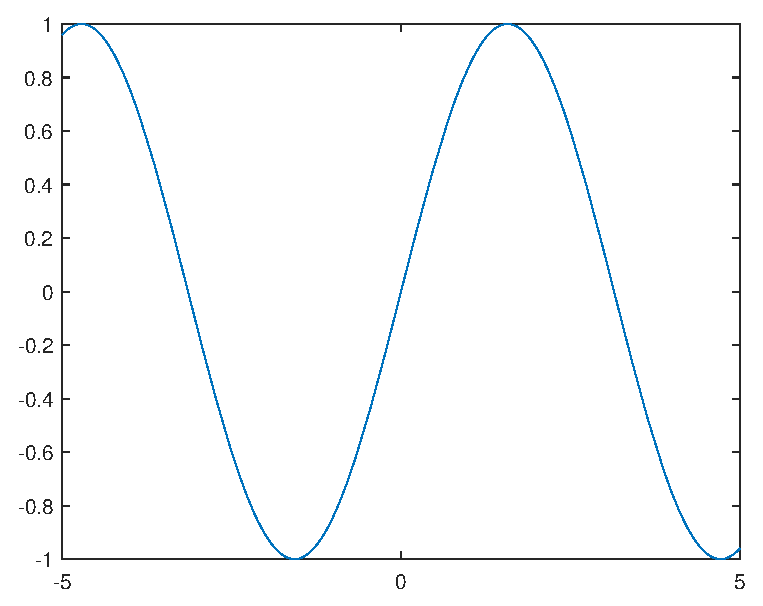
\includegraphics[width=7.2cm]{image1}
  \caption{函数 $y=\sin(x)$ 的图像}\label{fig:sinx}
\end{figure}

两个图左右并排放置, 共用一个标题, 如图~\ref{fig:image}.
\begin{figure}[htp!]
  \centering
  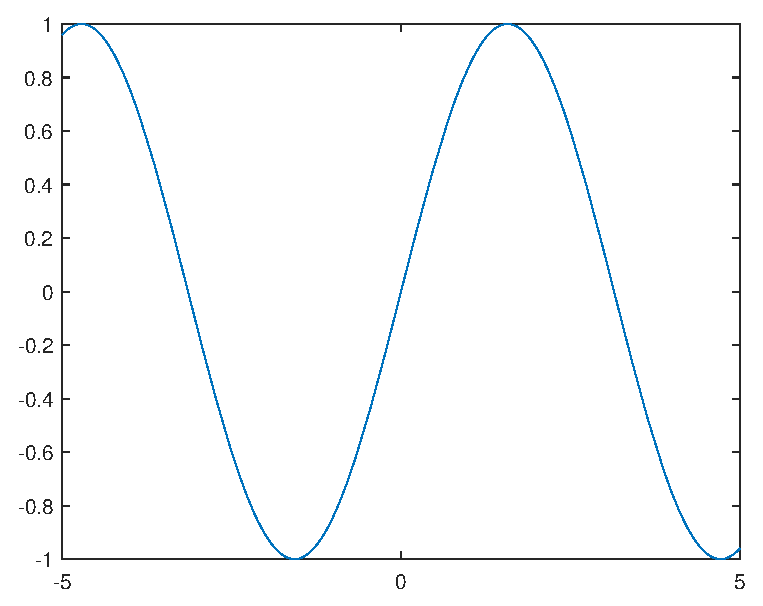
\includegraphics[width=0.45\linewidth]{image1}
  \hfill
  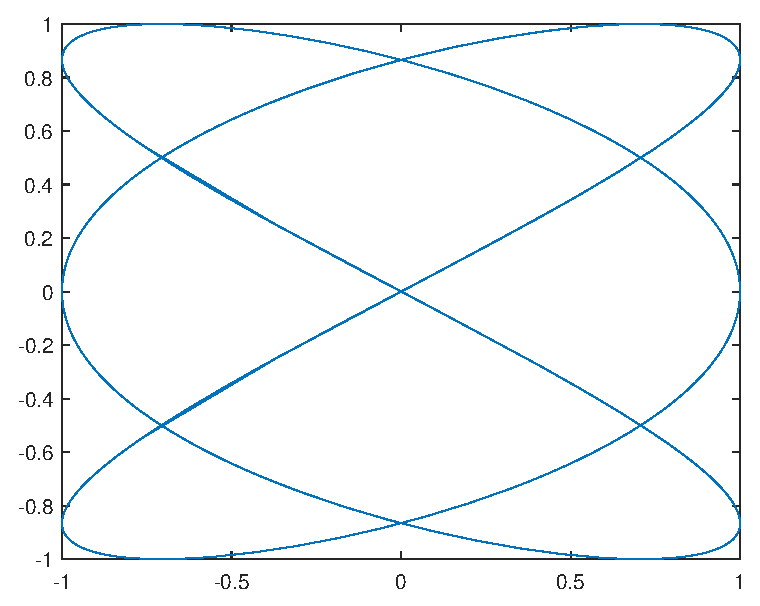
\includegraphics[width=0.45\linewidth]{image2}
  \caption{左: 图一的描述;~ 右:图二的描述}
  \label{fig:image}
\end{figure}

\clearpage
使用 minipage 排版并排插图, 每个图都有单独的标题. 通过 \verb|autoref| 引用图片: \autoref{fig:image1} 与 \autoref{fig:image2}.
\begin{figure}[htp!]
\begin{minipage}[t]{0.48\linewidth}
  \centering
  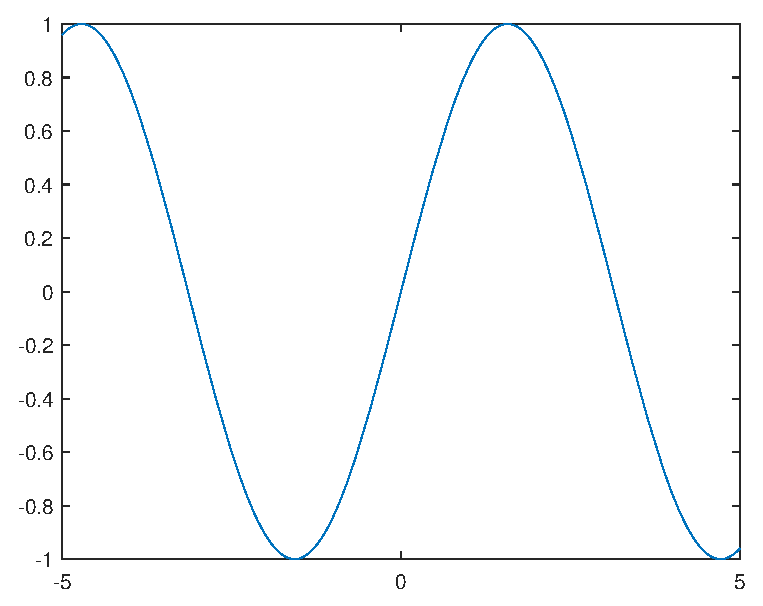
\includegraphics[width=0.9\linewidth]{image1}
  \caption{图一的描述}
  \label{fig:image1}
\end{minipage}
\hfill
\begin{minipage}[t]{0.48\linewidth}
  \centering
  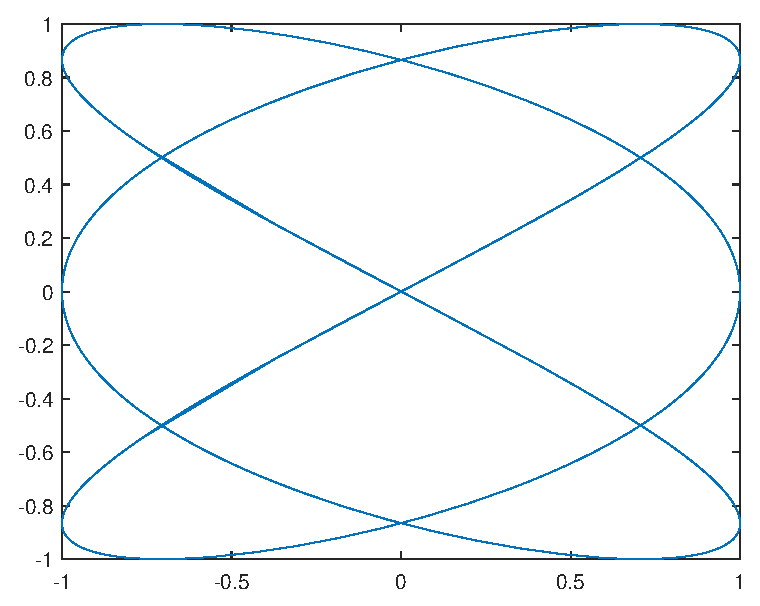
\includegraphics[width=0.9\linewidth]{image2}
  \caption{图二的描述}
  \label{fig:image2}
\end{minipage}
\end{figure}

使用 subfig 宏包实现多图并排, 如图~\ref{fig:images}.
\begin{figure}[htp!]
\centering
\subfloat[Subcaption A]{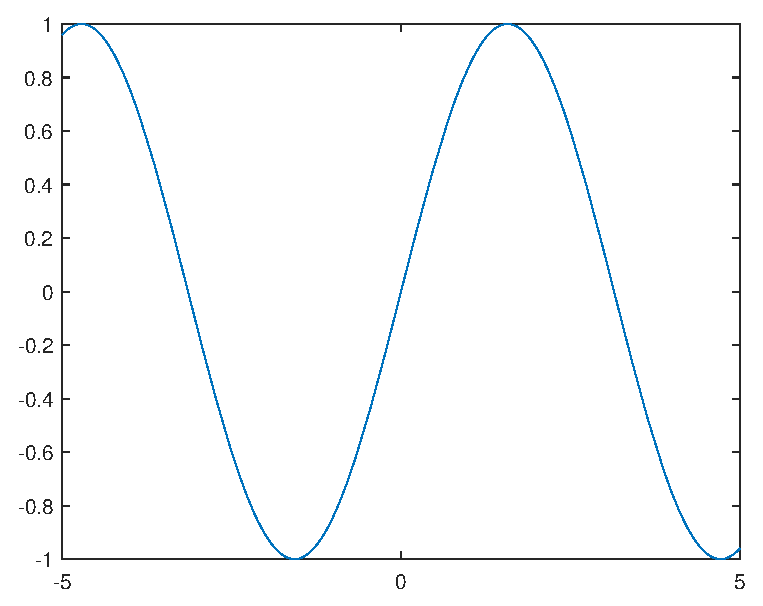
\includegraphics[width=0.3\linewidth]{image1}}
\hfill
\subfloat[Subcaption B]{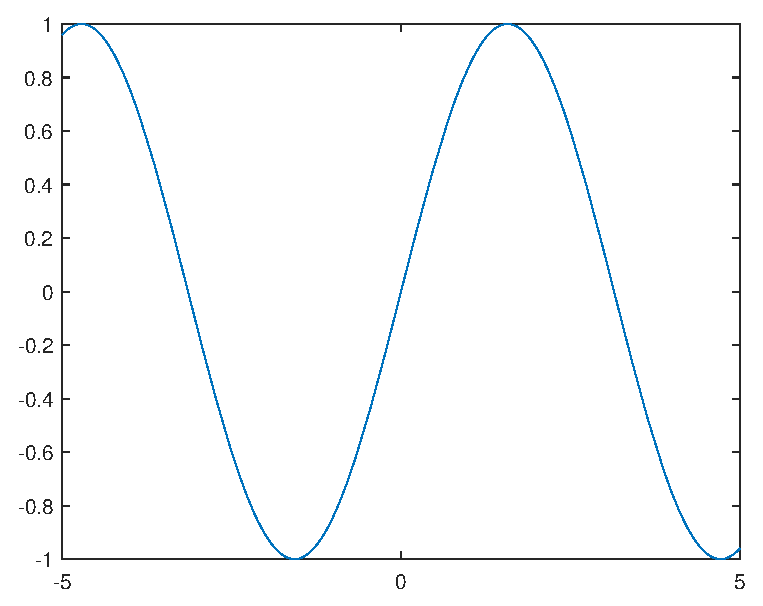
\includegraphics[width=0.3\linewidth]{image1}}
\hfill
\subfloat[Subcaption C]{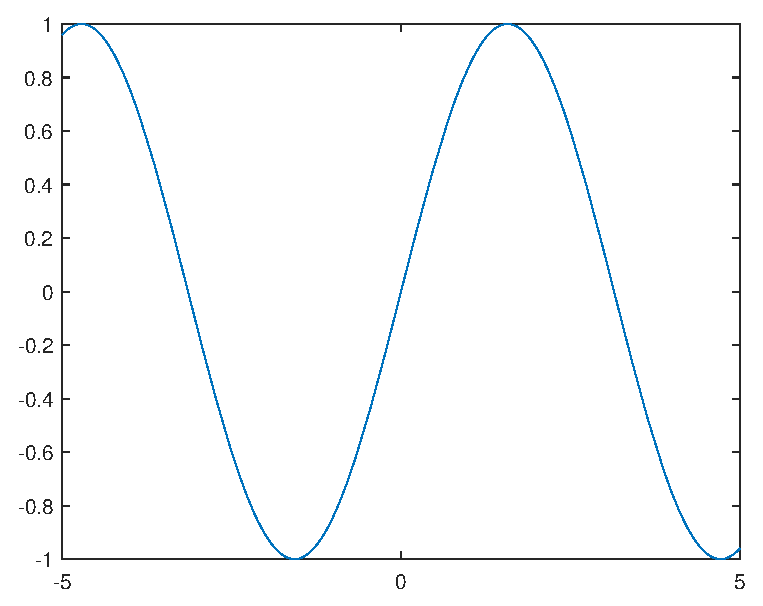
\includegraphics[width=0.3\linewidth]{image1}} \\
\subfloat[Subcaption D]{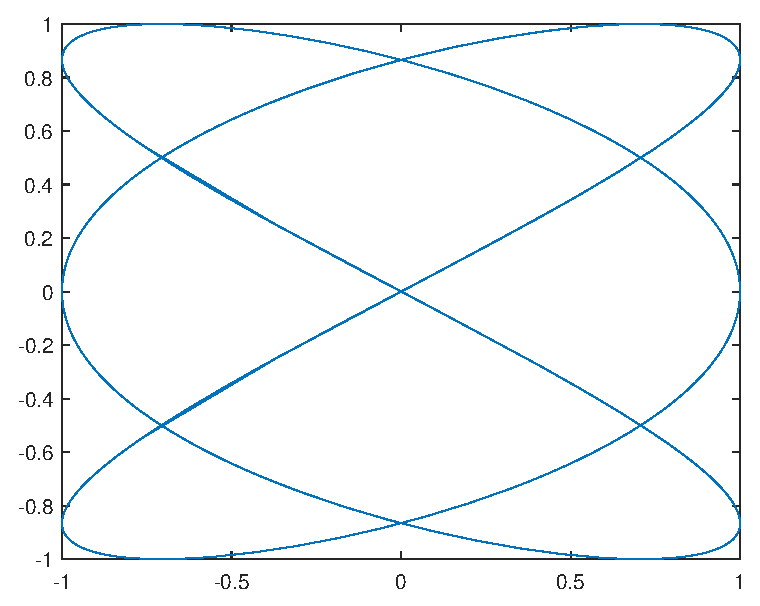
\includegraphics[width=0.3\linewidth]{image2}}
\hfill
\subfloat[Subcaption E]{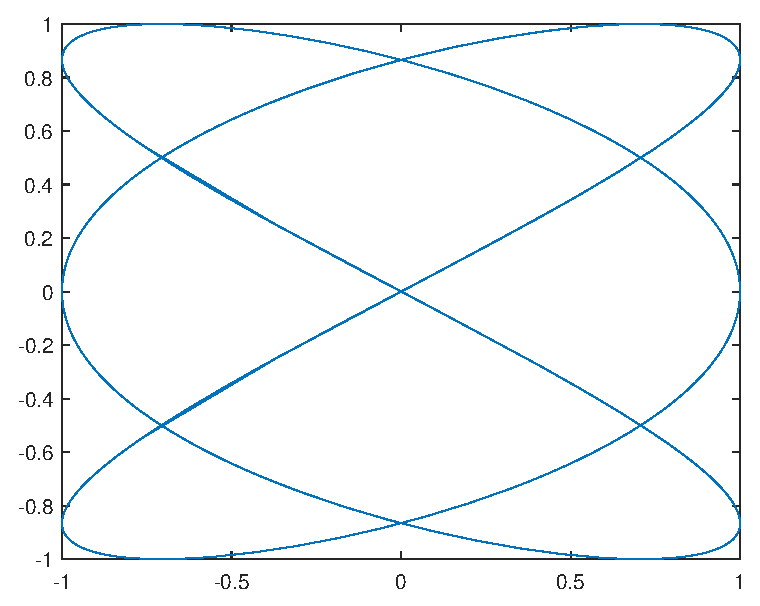
\includegraphics[width=0.3\linewidth]{image2}}
\hfill
\subfloat[Subcaption F]{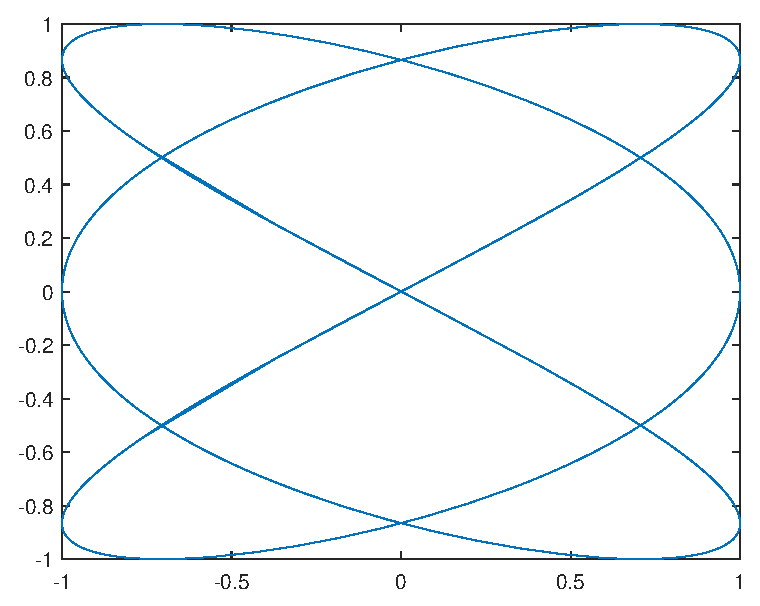
\includegraphics[width=0.3\linewidth]{image2}}
\caption{六个图并排}
\label{fig:images}
\end{figure}

